\section{Proposed Solution}
\label{sec:proposed_solution}

Our objective is to address the limitations associated with the current centralized cloud computing model by transitioning certain aspects of it to a decentralized model. In this model, independent entities, known as node providers, can host and execute arbitrary workloads on their servers, similar to the execution of Web3 smart contracts.

However, unlike Web3, where potential malicious behavior is countered by replicating the same workload across multiple nodes and running consensus on the execution outcome, our model takes a different approach. While replication and consensus are effective, they come with a high cost in terms of data transfer and time, especially when the nodes are geographically distributed.

\subsection{Leveraging Reputation}

Traditional cloud computing operates without major problems, and instances of malicious behavior among cloud providers are rare. This is because cloud providers have made significant investments to start operating and have their reputation at stake if they offer subpar service.

Our solution is to implement a robust method for tracking the reputation of all participants, making it highly undesirable for a participant to risk losing their hard-earned reputation. This approach nearly eliminates the risk of malicious behavior. A node provider might accept or reject running a workload based on the developer reputation, and vice versa.

\subsection{Decentralized Matching Engine for Efficient Resource Allocation}

To ensure efficient resource allocation and task scheduling, the platform will use a modern matching engine and, if needed, machine learning algorithms. Resource matching will among other things consider factors such as the task requirements, the resources of each node, the network conditions, and the reputation of the nodes.
This approach allows for dynamic load balancing among node providers based on demand. Moreover, by implementing robust security measures and a reputation system, the system will be secure and trustworthy.

\subsection{Affordable nodes. Security included.}

The demand for nodes from developers is easily met by supply provided by node providers. Our decentralized cloud platform is designed to operate independently of blockchain performance constraints. The matching engine that runs as a smart contract only stands on the control path of node usage -- finding and contracting a suitable node, thereby ensuring that the performance of the platform is not limited by the blockchain's capabilities.

All developers will need nodes, and node providers have more than enough nodes to handle the demand. Our matching engine is only used for signing the contract, which means that blockchain performance does not limit the performance of the decentralized cloud platform.

For some use cases, such as storing and rotating tokens, certificates, and other secrets, developers will need nodes with additional security. For these use cases, platform will support Confidential Containers\cite{brasser2022trusted}.

\subsection{Wide Range of Applications}

The platform will support a wide range of applications, from scientific computing and machine learning to web hosting and data storage. By providing a decentralized alternative to traditional cloud providers, the platform will promote competition in the cloud computing market and drive down prices.

\subsection{DAO Governance}

By employing a decentralized matching engine and a DAO model for governance, we aim to create a system that is transparent and democratic, fostering competition and innovation.


Figure~\ref{fig:proposed-architecture} illustrates the architecture of the proposed platform. In the following sections we'll dive into details on each of the above topics.


\begin{figure*}[h]
    \centering
    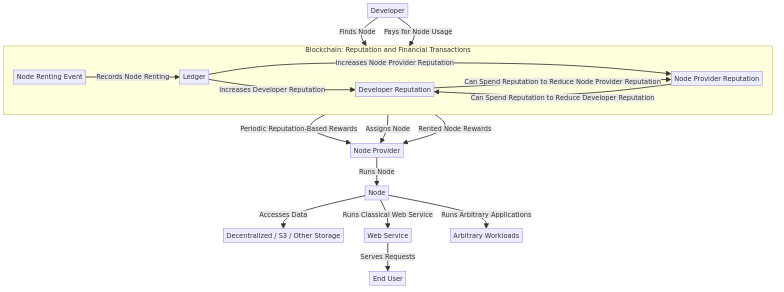
\includegraphics[width=\textwidth]{figures/proposed_architecture.png}
    \caption{Proposed platform architecture.}
    \label{fig:proposed-architecture}
\end{figure*}
